\chapter{Novel Work}

In this section the work completed so far will be presented. Two main areas of the systematic review process has been focused on. Stopping criteria and indexing/querying pubmed.

\section{Random Sample Method to Stopping}

As approach to determining when to stop looking at document abstracts returned by the query we are proposing a new sampling method. This approach assumes we have optimum ranking algorithm for returning documents for a query.

The first step of this method is to randomly sample a returned set of documents into a subsets. 

\begin{equation}
U = \frac{|D|}{S}
\end{equation}

Where $U$ is the computed randomised subset, $D$ is the document collection and $S$ is the sample size.

We then use this subset $U$ to create a model / baseline for our topic as a way of predicting how many documents one would need to look at to hit a threshold. The intuition behind this approach is that the rate of which relevant documents occur should be relatively similar when the number of returned documents in the same.

A limitation of this sampling method is that for topics with very few documents it is easy for a sample to miss many of them. This creates a subset set bias, where one set contains a larger percentage of relevant documents. Consider a query that returns 10000 candidate documents of which only 10 have been pre-determined to be relevant. Its not too unlikely that a randomly sampled subset would contain 0 relevant documents. We can use the following equation to tell us how much information we can take from a pre-evaluated topic:

\begin{equation}
I = \frac{rel(T_i)}{|T_i|}
\end{equation}

Where $T_i$ is a given topic and $rel$ computes the number of relevant documents for that topic. Therefore $I$ is telling us how useful the topic is at fitting a curve. We can take the average simply by taking the mean of $I$ across all topics:

\begin{equation}
Usefullness = \frac{\sum{I}}{|T|}
\end{equation}



\subsection{Curve Fitting}

Our first approach uses a simple curve fit against a sample set along with a simple non-linear function. $f(x)$

\begin{equation}
F(x) = n - a\exp^{-kx}
\end{equation}

Where $a$, $k$ and $n$ are learnt weights and $x$ is an associated return rate for a document.

We can visualise the curve along with the confidence intervals. The Y axis is the predicted number of relevant documents for the topic. X axis shows the true number of documents returned for the query. 

\begin{figure}[H]
\center
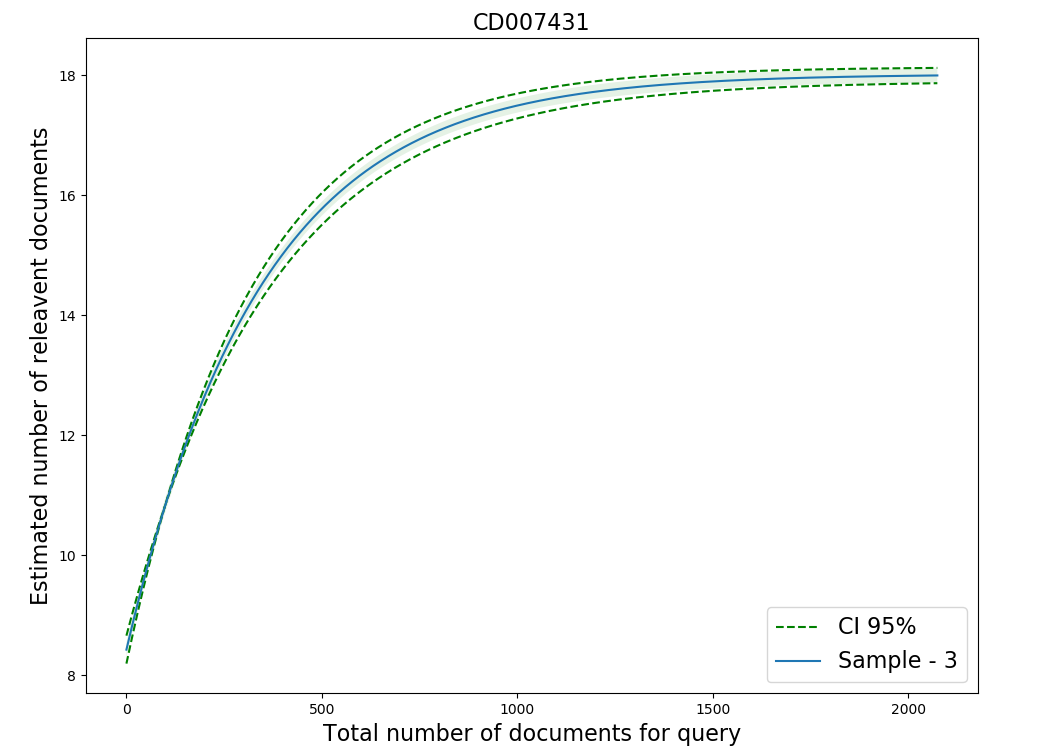
\includegraphics[width=10cm]{figures/curve_fit_example.png}
\caption{Example of fitting a curve for a topic using sampling}
\end{figure}

\begin{table}[H]
\centering
\begin{tabular}{|c|c|c|c|} 

 \hline
 sample size & recall & reliability & effort  \\ 
 1 & 0.91 &	0.96	&	1 \\ 
 3 & 0.66 & 0.5	&	0.48 \\ 
 5 & 0.481 & 0.33	&	0.315 \\ 
 \hline
\end{tabular}
\caption{Comparison of different sample sizes against recall and effort. Ranking Method: Test\_Data\_Sheffield-run-2 \cite{Alharbi2017}}

\end{table}

The first sample size of 1 is included to show how the effort metric is effected. For us to use sample everything, we would need to look at everything, as such the effort averaged out at 1. In this example we were only concerned in achieving 70\% recall, as such even when sampling everything we would really obtain 100\% recall at the expense of 100\% effort.

Looking at every 3rd document and then producing a prediction curve will reduce our effort. We are still required to look at at 1/3 of documents, as such the effort will always be above 0.33. 

\subsubsection{Relevance Ranking}

Our results so far have been based on Test\_Data\_Sheffield-run-2 \cite{Alharbi2017} of CLEF 2017. Naturally, the reliability of our curve is heavily based on how good the initial rankings are for each topic. We can compare different ranking methods for generating our stopping curve. By looking at the CLEF 2017 technology assisted review task \cite{Kanoulas12017} we can determine the best candidates to use. We introduce an additional field of topics sampled as some of the ranking methods do not produce enough relevant documents to generate a suitable curve.


\begin{table}[H]
\centering
\begin{tabular}{|c|c|c|c|c|} 

 \hline
 Submission & recall & reliability & effort & topics sampled [Max 30]  \\ 
 Test\_Data\_Sheffield-run-2 & 0.66 &	0.5	&	0.48 & 30 \\ 
 Waterloo A-rank-cost & 0.65 & 0.41	&	0.39 & 29 \\ 
 Waterloo B-rank-cost & 0.70 & 0.46	&	0.40 & 30 \\ 
 auth run-1 & 0.71 & 0.5	&	0.41 & 30 \\ 
 auth run-2 & 0.67 & 0.46	&	0.40 & 30 \\ 
 ntu run-1 & 0.56 & 0.18	&	0.54 & 22 \\ 
 ucl full-text & 0.55 & 0.36	&	0.70 & 11 \\ 
 \hline
\end{tabular}
\caption{Comparison of different of sample method using curve fitting for different CLEF 2017 runs. Sample size = 3. Results are taken as averages over all topics for search method}

\end{table}

We have deliberately compared two of the better participant rankings (Waterloo and auth) and two of the lower performers (ntu and ucl). We can see the quality of the initial rankings significantly influences the performance of our stopping criteria. This suggests there is a important relationship between using a curve to predict a stopping point and how good the initial ranking of documents is.

\subsection{Gaussian Process fitting}

As an alternate approach to fitting a simple curve, we can apply a GP.

We will apply a constant kernel plus a squared-exponential kernel.

\begin{table}[H]
\centering
\begin{tabular}{|c|c|c|c|c|} 

 \hline
 Submission & recall & reliability & effort & topics sampled [Max 30]  \\ 
 Test\_Data\_Sheffield-run-2 & 0.694 &	0.66	&	0.49 & 30 \\ 

 \hline
\end{tabular}
\caption{Comparison of different of sample method using GP fitting for different CLEF 2017 runs. Sample size = 3. Results are taken as averages over all topics for search method.}

\end{table}
